\begin{pastexam}[label={px:ust-112-ee-ds-08}]{臺聯大電機類 112 學年度 第 8 題}
（單選；3 分）

Consider the given graph, what is the weight of the minimum spanning tree using the Prim's
algorithm, starting from vertex a?

\begin{center}
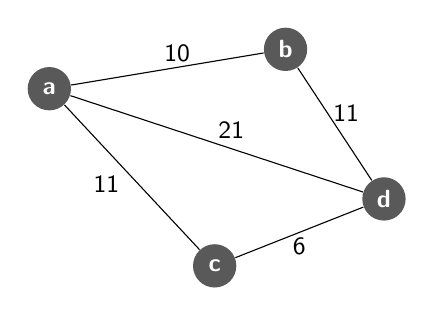
\begin{tikzpicture}[v/.style={circle,fill=black!65,text=white,font=\sffamily\bfseries\small,inner sep=1.5pt,minimum size=5.5mm},
  w/.style={font=\sffamily\small,inner sep=2pt}]
\node[v] (a) at (0,0) {a};
\node[v] (b) at (3,0.5) {b};
\node[v] (d) at (4.25,-1.4) {d};
\node[v] (c) at (2.1,-2.25) {c};
\draw (a) -- node[w,above,pos=0.55] {10} (b);
\draw (b) -- node[w,right,pos=0.4] {11} (d);
\draw (a) -- node[w,above,pos=0.55,yshift=1.5pt] {21} (d);
\draw (a) -- node[w,below left,pos=0.45] {11} (c);
\draw (c) -- node[w,below,pos=0.5] {6} (d);
\end{tikzpicture}
\end{center}

(A)~23 \qquad (B)~28 \qquad (C)~27 \qquad (D)~11
\end{pastexam}

\begin{pastsoln}
答案是 (C) 27。

Prim 演算法從 $a$ 開始，每一步加入「一端在樹內、一端在樹外」的邊裡權重最小的那一條
（資結書第~24.3~節）。 圖的邊：$ab = 10$、$ac = 11$、$ad = 21$、$bd = 11$、$cd = 6$。

\begin{center}
\begin{tabular}{clll}
\toprule
步驟 & 樹內頂點 & 候選邊（跨越樹內外） & 加入 \\
\midrule
1 & $\{a\}$ & $ab = 10$、$ac = 11$、$ad = 21$ & $ab = 10$ \\
2 & $\{a, b\}$ & $ac = 11$、$bd = 11$、$ad = 21$ & $ac = 11$（和 $bd$ 同分，任選） \\
3 & $\{a, b, c\}$ & $cd = 6$、$bd = 11$、$ad = 21$ & $cd = 6$ \\
\bottomrule
\end{tabular}
\end{center}
總權重 $10 + 11 + 6 = 27$。 第 2 步若改選 $bd = 11$，第 3 步就加入 $cd = 6$，總和一樣是 $27$；
同分時選哪一條只影響樹的形狀，不影響最小權重。

檢查：$4$ 個頂點的生成樹有 $3$ 條邊。 最便宜的三條是 $6, 10, 11$，而 $\{cd, ab, ac\}$ 不成環，
所以 $27$ 已經是所有生成樹權重的下界，也就是最小值。 (A) 23、(D) 11 比三條最小邊的和還小，
不可能；(B) 28 不是最小。
\end{pastsoln}
